\documentclass[12pt,a4paper,oneside]{article}
\usepackage{amsmath,amsthm}
\usepackage{graphicx}
\usepackage{ctex}
\usepackage{float}
\usepackage{subfigure,subcaption}
\usepackage{caption}
\usepackage{geometry}

\geometry{a4paper,scale=0.8}

\title{计算方法编程作业6实验报告}
\author{张博厚 PB22071354}
\date{}

\begin{document}
\maketitle
\section{实验目的}
通过快速傅里叶变换和快速傅里叶逆变换实现对给定函数的Fourier分析及重建,分析采样数目
、去除高频系数对函数重建的影响。


\section{问题描述与算法}
\subsection{快速傅里叶(逆)变换}
快速傅里叶变换与快速傅里叶逆变换的算法伪代码由教材及实验文档附录给出,如下所示:
\begin{figure}[H]
    \centering
    \subfigure[FFT算法]{
        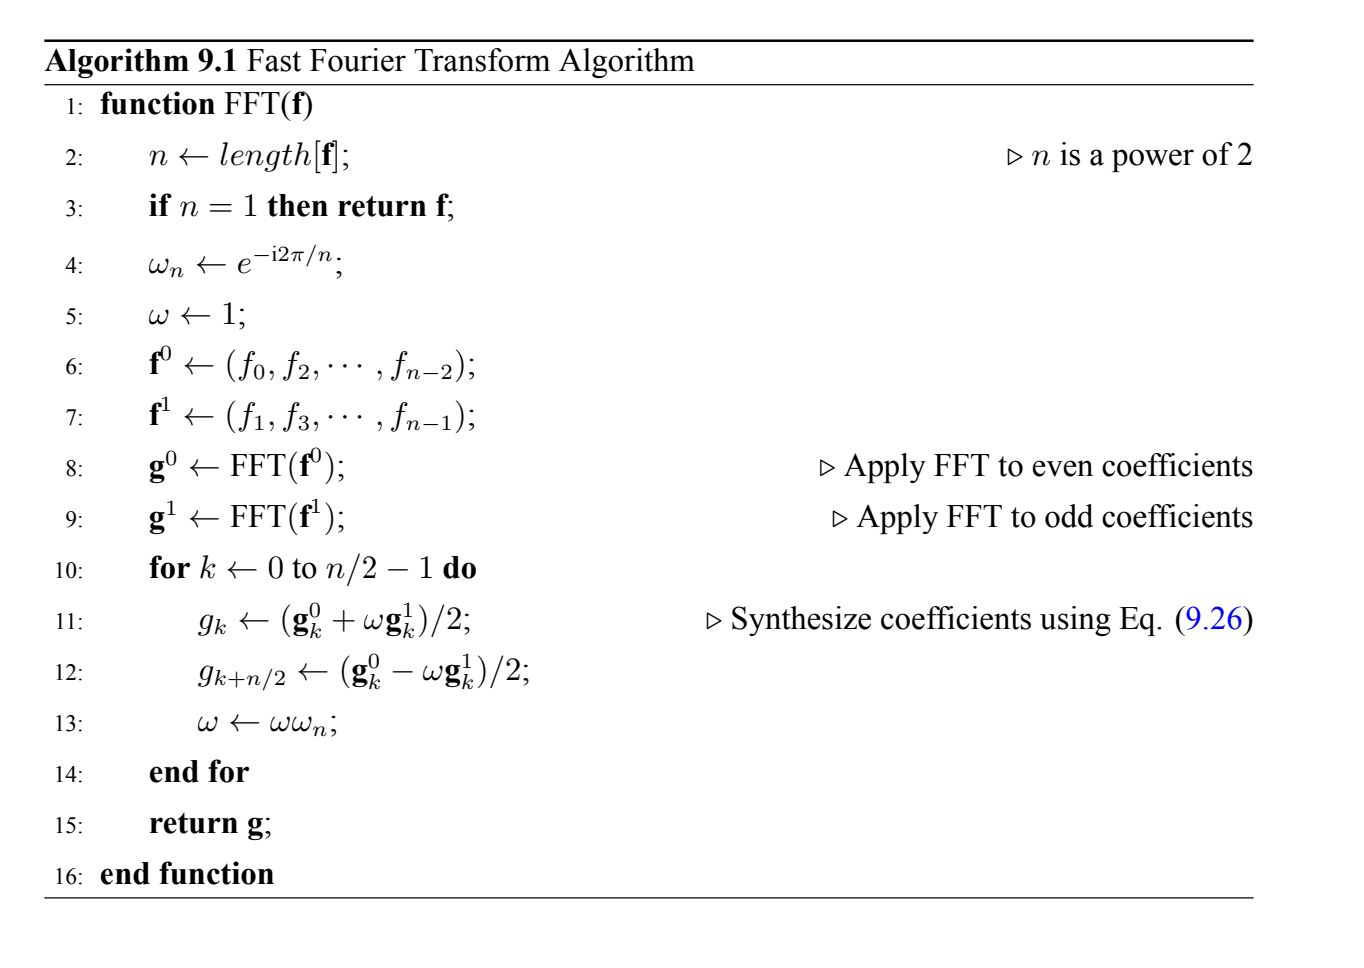
\includegraphics[width = 0.4\textwidth]{figs/FFT_algo.jpg}
    }
    \subfigure[IFFT算法]{
        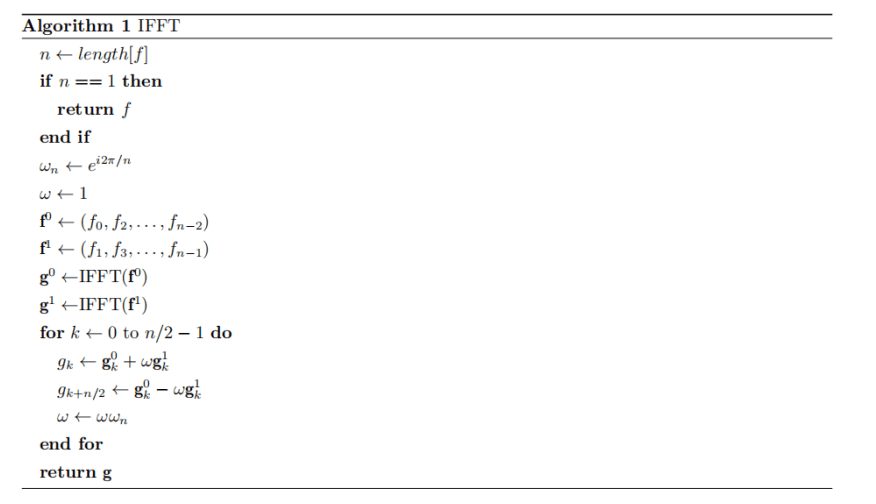
\includegraphics[width = 0.5\textwidth]{figs/IFFT_algo.png}
    }
\end{figure}
比较两图不难发现,FFT与IFFT算法十分相似,在实现时可作为同一个函数来编写,并由一参数
NonInverse来标识区分即可。

\subsection{数据可视化}
数据可视化部分使用python+matplotlib实现,通过对实验要求的分析,可知共需绘制以下三种图像:
\paragraph{1} 对于函数f与频率n,对f执行快速傅里叶变换FFT(f, n),绘制执行后的结果$|g_i|$与频率
的关系。
\paragraph{2} 对f,频率n,执行FFT后的结果g,对g作快速傅里叶逆变换IFFT(g,n),将所得结果与
f作比较,绘制到同一张图里。
\paragraph{3} 特别地,对于f2,还需取经FFT后频率域前25\%的系数作IFFT,并和f2进行比较。\\ \par
对于f2,上述2,3图像可绘制到同一张图内。由于python不支持本地函数重载,共需编写三个函数,分别
对应上述三种图像。

\section{实验结果}
\subsection{输出结果}
对于f1, $n=2^4$, 结果为:
\begin{figure}[H]
    \centering
    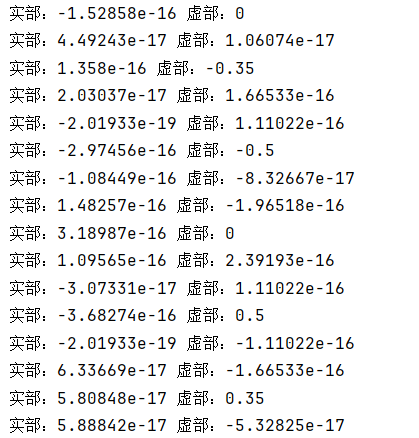
\includegraphics[scale = 0.5]{figs/f1_1.png}
    \caption{$f1,n=2^4$结果}
\end{figure}
对于f1, $n=2^7$, 结果为:
\begin{figure}[H]
    \centering
    \subfigure{
        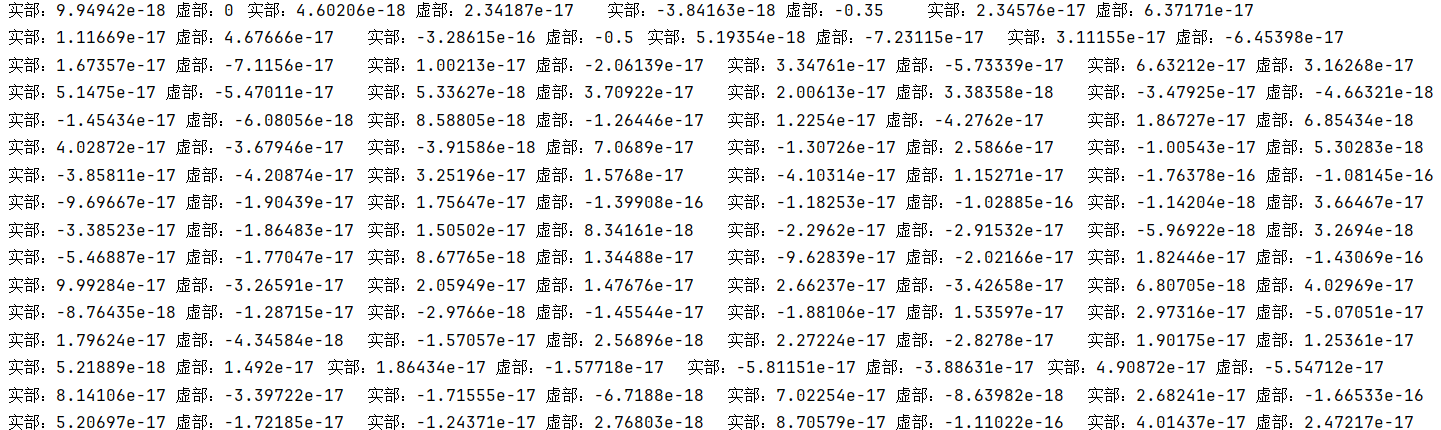
\includegraphics[width = \textwidth]{figs/f1_2_1.png}
    }
    \subfigure{
        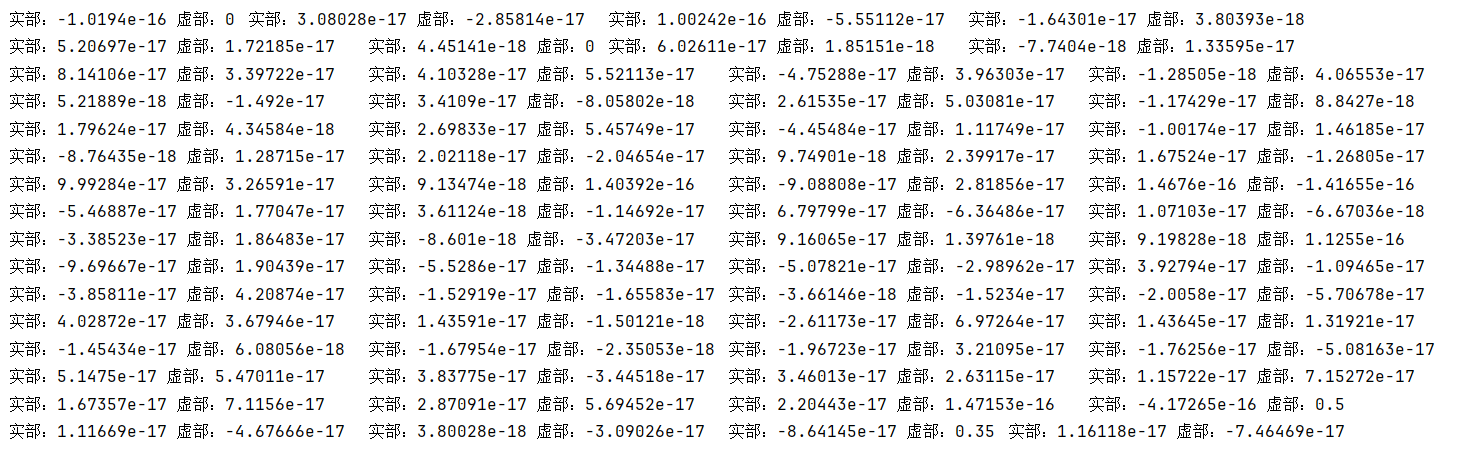
\includegraphics[width = \textwidth]{figs/f1_2_2.png}
    }
    \caption{$f1,n=2^7$结果}
\end{figure}
对于f2,结果为:

\begin{figure}[H]
    \centering
    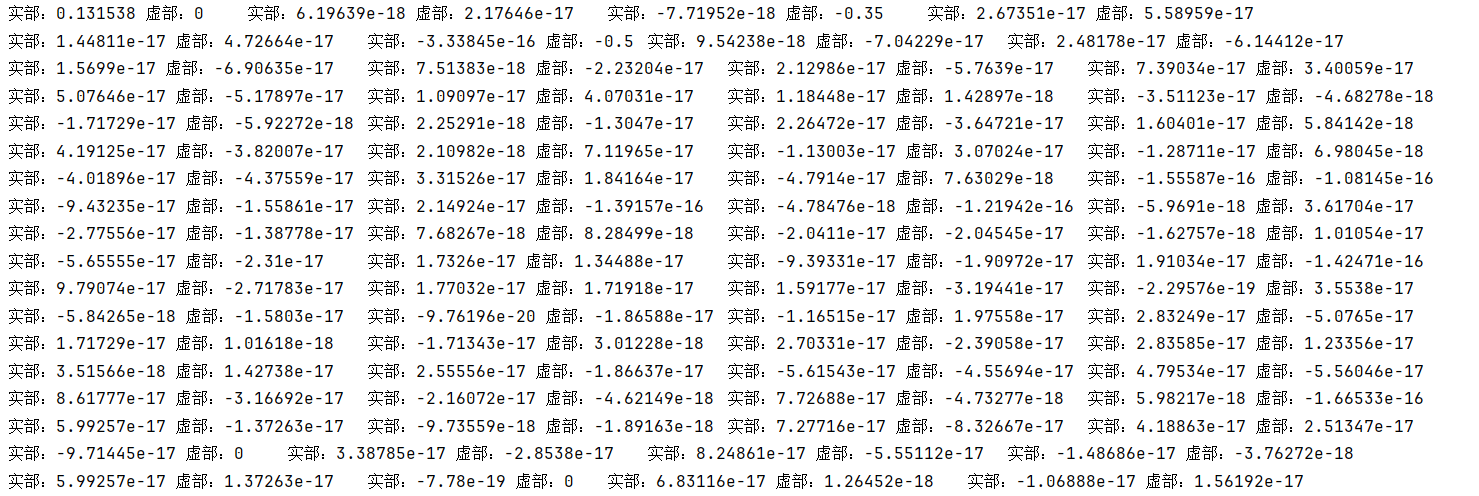
\includegraphics[width = \textwidth]{figs/f2_1.png}
    \caption{f2结果第一部分}
\end{figure}

\begin{figure}[H]
    \centering
    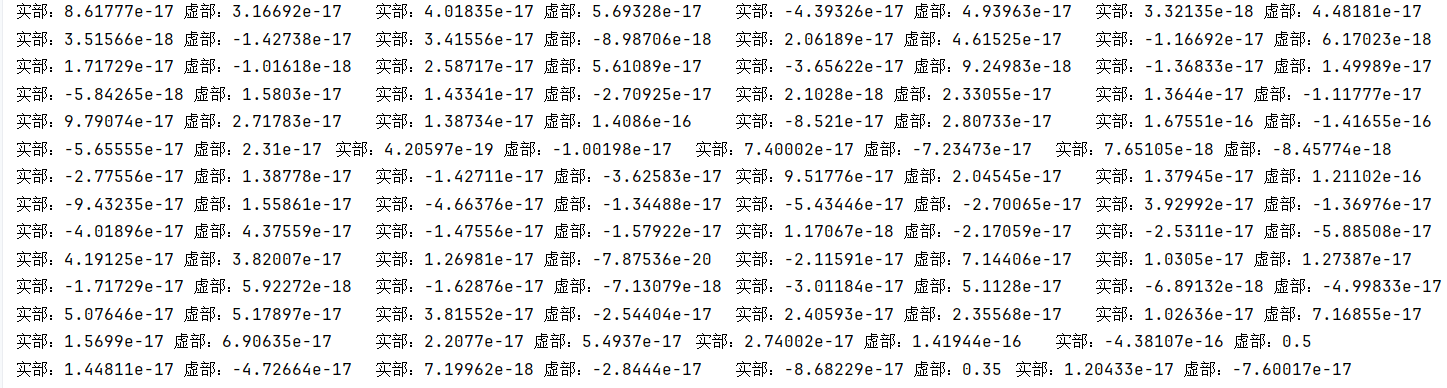
\includegraphics[width = \textwidth]{figs/f2_2.png}
    \caption{f2结果第二部分}
\end{figure}

\subsection{绘制实验图像}
\subsubsection{FFT结果图像}
$f1, n=2^4:$
\begin{figure}[H]
    \centering
    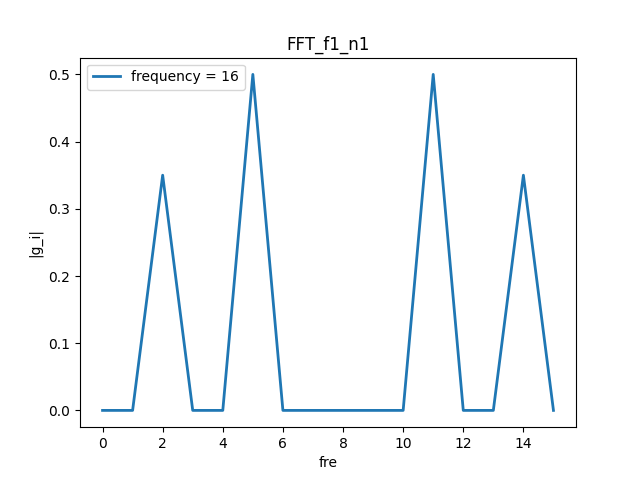
\includegraphics[scale = 0.85]{../res/figs/FFT_f1_n1.png}
\end{figure}
从图像可知,结果满足共轭对称性,在频率为2Hz(14Hz), 5Hz(11Hz)处取得振幅峰值,其他频率
处振幅最小。振幅峰值分别为0.35,0.5,即各自为f1峰值0.7与1的一半,与预期符合得较好。
\par
$f1, n = 2^7:$
\begin{figure}[H]
    \centering
    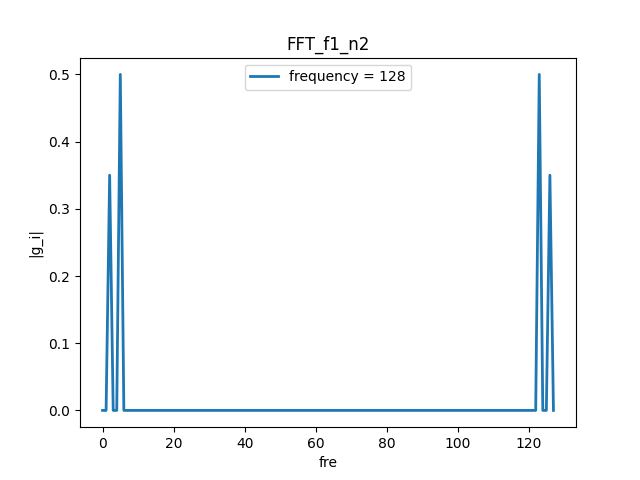
\includegraphics[scale = 0.85]{../res/figs/FFT_f1_n2.png}
\end{figure}
与频率为$2^4$时类似,仍在频率为2Hz、5Hz及他们的对称位置取得振幅峰值,峰值仍分别为0.35,
0.5.\par
$f2,n = 2^7$:
\begin{figure}[H]
    \centering
    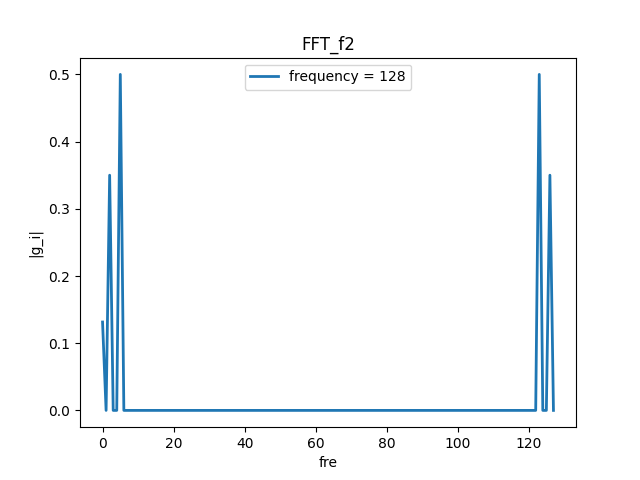
\includegraphics[scale = 0.85]{../res/figs/FFT_f2.png}
\end{figure}
\par
可以看出,假如随机扰动之后,结果在一定程度上不再满足共轭对称性(如0Hz处),但仍然满足
在频率为2Hz、5Hz及他们的对称位置取得振幅峰值,峰值仍分别为0.35,0.5.这说明在带有噪声
影响的情况下,FFT仍然适用。

\subsection{原图与重建后图像对比}
$f1, n = 2^4$:
\begin{figure}[H]
    \centering
    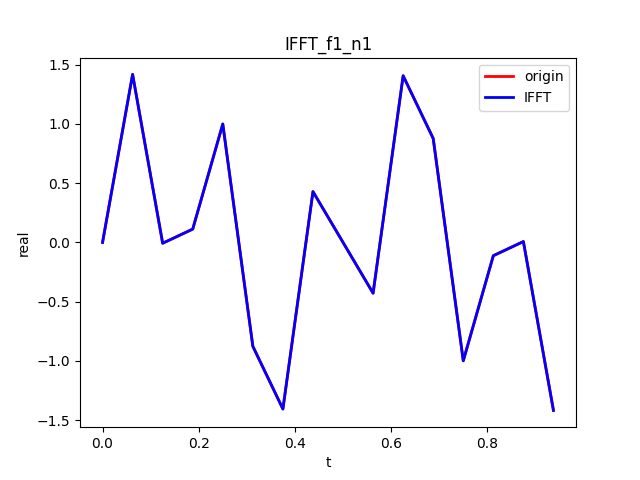
\includegraphics[scale = 0.85]{../res/figs/IFFT_f1_n1.png}
\end{figure}
$f1, n = 2^7$:
\begin{figure}[H]
    \centering
    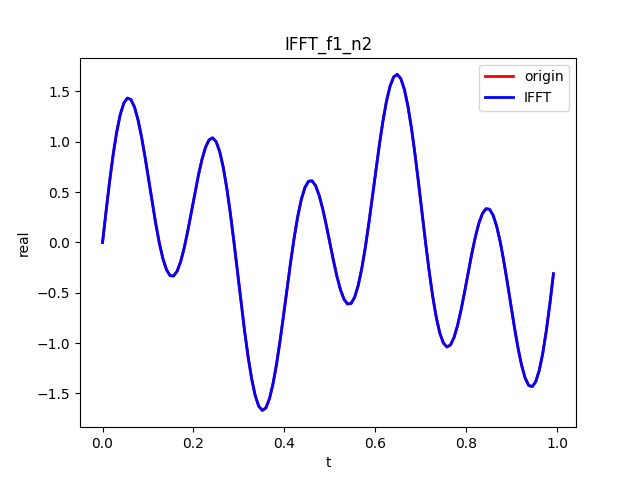
\includegraphics[scale = 0.85]{../res/figs/IFFT_f1_n2.png}
\end{figure}
$f2, n = 2^7$:
\begin{figure}[H]
    \centering
    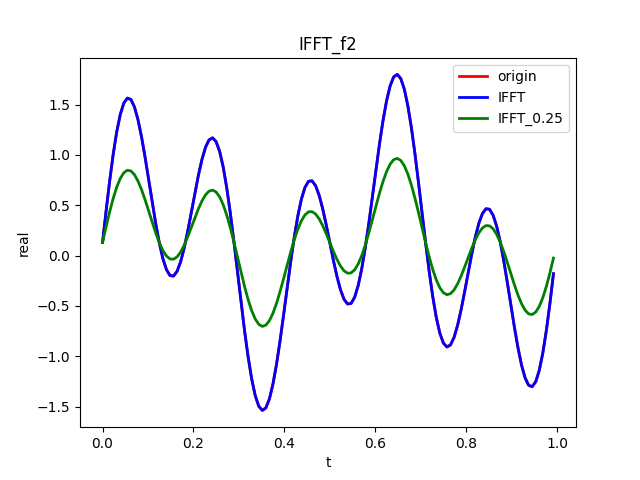
\includegraphics[scale = 0.85]{../res/figs/IFFT_f2.png}
\end{figure}

\section{结果分析}\noindent
1.采样数对结果影响:采样数目越多,结果点数相应也越多,体现在图像上更加光滑,准确程度更好。
但此次实验中,f1在选取两种n情况下,原图像与重建后图像均符合较好,因此采样数对该项的影响
并未有明显体现。\\
2.对f2,去掉高频系数后使得结果振幅缩小为原本的一半。此外图像更光滑、更接近f1,一定程度上起到了去噪
的作用。

\end{document}